\documentclass[10pt, a4paper]{article}
\setlength{\leftmargini}{0.75cm}
\setlength{\parindent}{0.0cm}
\setlength{\parskip}{0.2cm}
\setlength{\topsep}{0.0cm}
\usepackage{color,fancyhdr}
\usepackage[top=2.4cm, bottom=2.4cm, left=2.4cm, right=2.4cm]{geometry}
\usepackage{graphicx,amsmath,amssymb,subfigure}
\usepackage[colorlinks=true,breaklinks=true,linkcolor=lightblue,citecolor=lightblue]{hyperref}

\newcommand{\cblue}[1]{\textcolor{lightblue}{#1}}
\definecolor{lightblue}{rgb}{0.22,0.45,0.70}
\newcommand\curl{\mathop{\mathrm{curl}}\nolimits}
\newcommand\bb{\boldsymbol{b}}
\newcommand\bu{\boldsymbol{u}}

\begin{document}

\sf 

\cfoot{}
\chead{}
\lfoot{\cblue{Monash Mathematics}}
\lhead{}
\rfoot{\cblue{C Thomopoulos / R Ruiz Baier}}
\rhead{}
\pagestyle{fancyplain}
\renewcommand{\headrulewidth}{0.0pt}
\begin{center}
\cblue{\hrule depth 0.5pt}
\vspace{-5pt}
\cblue{\hrule}
\vspace{-5pt}
\uppercase{\bfseries {\large S}ummer Research Project}\\
{Coupling of reaction-diffusion systems and rotational flows}\\
%\textbf{Semester 2, 2020}\\
\vspace{5pt}
\cblue{\hrule depth 0.5pt}
\vspace{3.0cm}~
\end{center}
\vspace{-3.5cm}

\section*{Project description} 
Reaction-diffusion systems can explain many phenomena taking place in diverse disciplines such as industrial and environmental processes, biomedical applications, population dynamics, etc.  These models allow to reproduce chaos, spatio-temporal patterns, rhythmic and oscillatory scenarios, and so on. Nevertheless, in most of the applications mentioned above, the reactions do not occur in complete isolation. The species are rather immersed in a fluid, or they move within (and interact with) a fluid-solid continuum. We want to perform linear stability analysis for a simplified coupled system to determine how the interaction between non-autonomous patterns arise in response to changes in the advecting fluid velocity and other flow conditions typical in rotation-based formulations. We also want to compute numerical solutions using advanced mixed finite element methods. 



\begin{figure}[h!]
\begin{center}
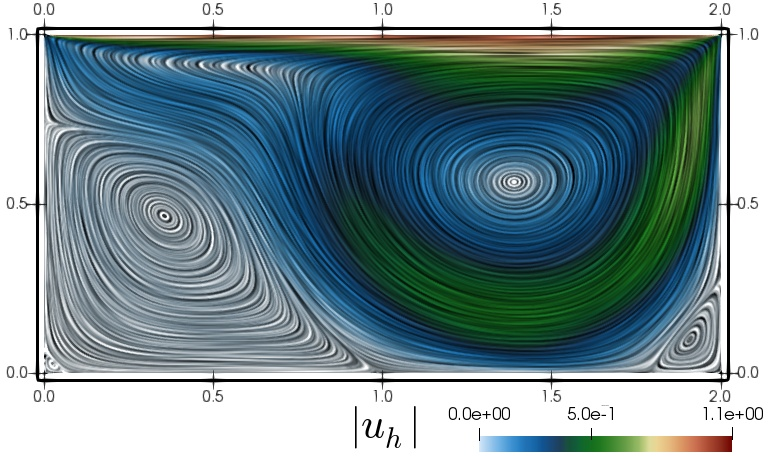
\includegraphics[width=0.45\textwidth]{ex02-lic}
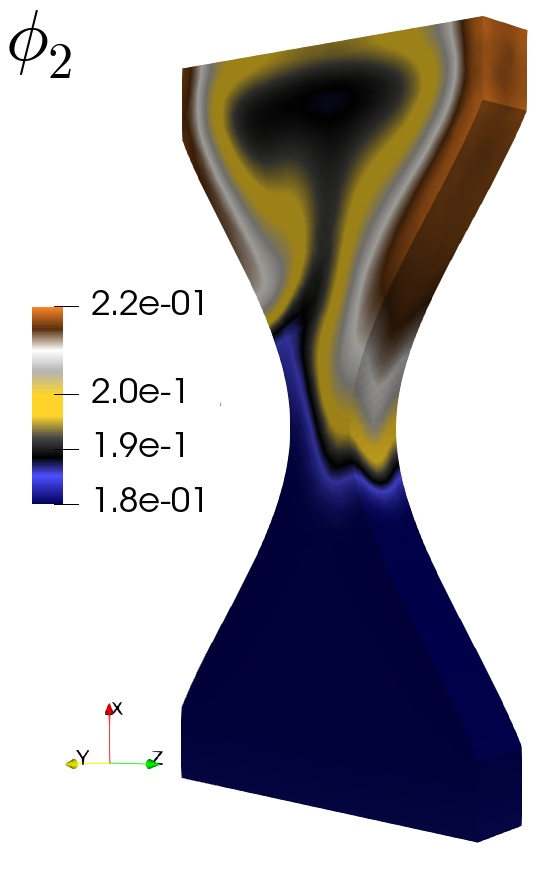
\includegraphics[width=0.175\textwidth]{ex03phi22}
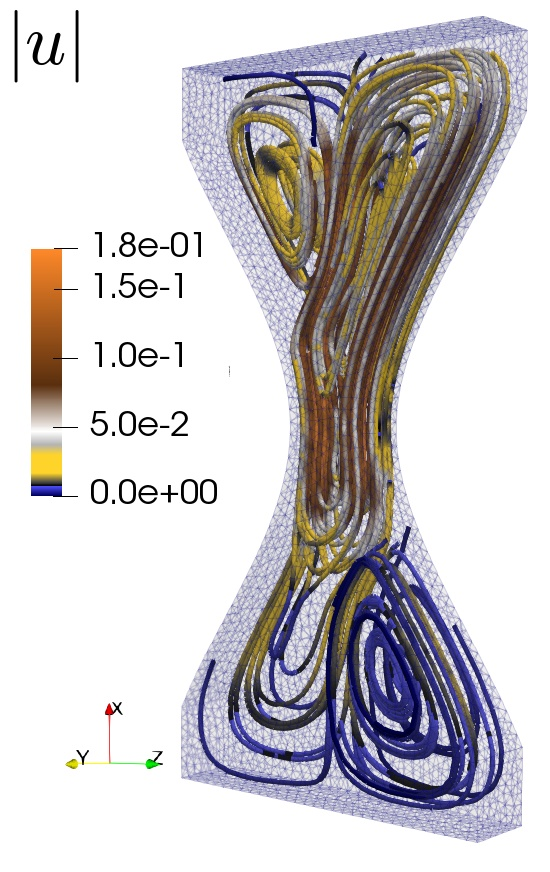
\includegraphics[width=0.175\textwidth]{ex03u2}
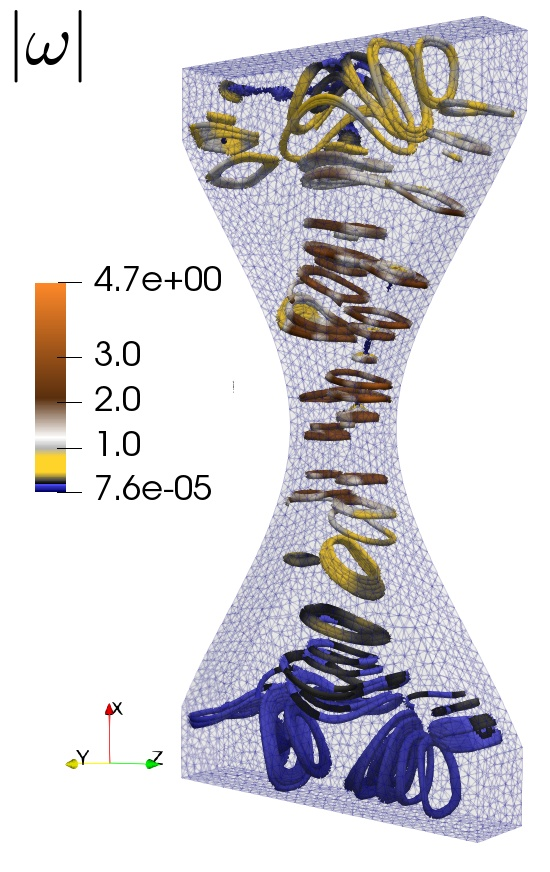
\includegraphics[width=0.175\textwidth]{ex03w2}
\end{center}
\label{fig:domains}
\end{figure}



Starting from the vorticity-velocity-pressure formulations from \cite{anaya19,anaya16}, we will write flow-transport coupled models based on a continuum representation of the solid phase and will replicate numerical results from e.g. \cite{alvarez}, using the open source finite element library FEniCS \cite{fenics}. 

Then we will replace the solid phase model by a discrete particle sedimentation approach and will adapt the existing implementation in \cite{leopart} to accommodate for vorticity-based formulations. Using Lagrangian particles for the discretisation of the advection operator permits to eliminate artificial dissipation, and therefore the framework is amenable for   simulating advection dominated flows. 



\begin{thebibliography}{99}
\small

 \bibitem{alvarez}
{\sc M. Alvarez, G.N. Gatica, and R. Ruiz-Baier},
{\it A posteriori error estimation for an augmented mixed-primal method applied to sedimentation-consolidation systems}. 
J. Comput. Phys., 367 (2018), pp.~322--346.

 \bibitem{anaya19} {\sc V. Anaya, A. Bouharguane, D. Mora,
C. Reales, R. Ruiz-Baier, N. Seloula, and H. Torres},
{\it Analysis and approximation of a vorticity-velocity-pressure
formulation for the Oseen equations}. J. Sci. Comput., 80(3) (2019)  1577--1606.


\bibitem{anaya16} {\sc V. Anaya, D. Mora, R. Oyarz\'ua, and
  R. Ruiz-Baier}, {\it A priori and a posteriori error
  analysis for a mixed scheme for the Brinkman problem}.
  Numer. Math., 133(4) (2016) 781--817.

\bibitem{garg} {\sc R. Garg, C. Narayanan, D. Lakehal, and S. Subramaniam}, {\it Accurate numerical estimation of interphase momentum transfer in Lagrangian-Eulerian simulations of dispersed two-phase flows}, Int. J. Multiph. Flow 33 (12) (2007) 1337--1364.

\bibitem{fenics} {\sc A. Logg, K.-A. Mardal, and G.N. Wells}, {\it Automated Solution of Differential Equations by the Finite Element Method}, Vol. 84, Springer Science \& Business Media, 2012. 

\bibitem{leopart} {\sc J.M. Maljaars, C.N. Richardson, and N. Sime}, {\it LEoPart: a particle library for FEniCS}. Arxiv preprint 1912.13375v2 [cs.MS] (2020).  

    \bibitem{olshanskii2015} {{\sc M.A. Olshanskii, T. Heister, L.G. Rebholz, and K.J. Galvin}, {\it Natural vorticity boundary conditions on solid walls}. Comput. Methods Appl. Mech. Engrg., 297 (2015) 18--37.}

\end{thebibliography}

\end{document}
